\section{Analysis of the Annealed Importance Sampling}
\label{sec:ais}
In practice, it is not feasible to simulate the ALD precisely, nor is it possible to evaluate the exact value of the work $W(X)$. Therefore, discretization and approximation are required. To address this, we first outline the following annealed importance sampling (AIS) equality akin to JE. 

\begin{theorem}[Annealed importance sampling equality \citep{neal2001annealed}] 
Suppose we have probability distributions $\pi_\l=\frac{1}{Z_\l}f_\l$, $\l\in\sqd{0,M}$ and transition kernels $F_\l(x,\cdot)$, $\l\in\sqd{1,M}$, and assume that each $\pi_\l$ is an invariant distribution of $F_\l$, $\l\in\sqd{1,M}$. Define the path measure
    \begin{equation}
        \Pr(x_{0:M})=\pi_0(x_0)\prod_{\l=1}^MF_\l(x_{\l-1},x_\l).
        \label{eq:ais_pr}
    \end{equation}
    Then the same relation between the work function $W$ and free energy difference $\Delta F$ holds:
    $$\E_{\Pr}\e^{-W}=\e^{-\Delta F},\quad\text{where}~~W(x_{0:M}):=\log\prod_{\l=0}^{M-1}\frac{f_\l(x_\l)}{f_{\l+1}(x_\l)}~~\text{and}~~\Delta F:=-\log\frac{Z_M}{Z_0}.$$
    \label{thm:ais}
\end{theorem}
\vspace{-1em}
\begin{proof}
    Since $\pi_\l$ is invariant for $F_\l$, the following backward transition kernels are well-defined:
    $$B_\l(x,x')=\frac{\pi_\l(x')}{\pi_\l(x)}F_\l(x',x),~\l\in\sqd{1,M}.$$
    By applying these backward transition kernels sequentially, we define the backward path measure
    \begin{equation}
        \Pl(x_{0:M})=\pi_M(x_M)\prod_{\l=1}^MB_\l(x_\l,x_{\l-1}).
        \label{eq:ais_pl}
    \end{equation}
    It can be easily demonstrated, as in \cref{eq:jar_rn}, that $\log\de{\Pr}{\Pl}(x_{0:M})=W(x_{0:M})-\Delta F$. Consequently, the identity $\E_{\Pr}{\de{\Pl}{\Pr}}=1$ implies the desired equality.
\end{proof}

To study non-asymptotic complexity guarantees, we focus on a widely used curve in theoretical analysis \citep{brosse2018normalizing,ge2020estimating}, which we refer to as the \emph{geometric interpolation}\footnote{\cref{eq:pi_theta} differs slightly from a widely used curve in applications \citep{gelman1998simulating,neal2001annealed}: $\pi_\theta\propto\pi^{1-\lambda(\theta)}\phi^{\lambda(\theta)}$, where $\phi$ is a prior distribution (typically Gaussian). We refer to both as \emph{geometric interpolation}.}:
\begin{equation}
    \pi_\theta=\frac{1}{Z_\theta}f_\theta=\frac{1}{Z_\theta}\exp\ro{-V-\frac{\lambda(\theta)}{2}\|\cdot\|^2},~\theta\in[0,1],
    \label{eq:pi_theta}
\end{equation}
where $\lambda(\cdot)$ is a decreasing function with $\lambda(0)=2\beta$ and $\lambda(1)=0$, referred to as the \emph{annealing schedule}. With this choice of $\lambda(0)$, by \cref{assu:pi}, the potential of $\pi_0$ is $\beta$-strongly-convex and $3\beta$-smooth, making sampling and normalizing constant estimation relatively easy. To estimate $Z_0$, we use the TI algorithm from \cite{ge2020estimating}, which requires $\Ot\ro{\frac{d^{\frac32}}{\varepsilon^2}}$ gradient oracle calls. In a nutshell, TI is an equilibrium method that constructs a series of intermediate distributions and estimates adjacent normalizing constant ratios via expectation under these intermediate distributions, realized through MCMC sampling from each intermediate distribution. As TI is peripheral to our primary focus, we defer its full description and complexity analysis to \cref{app:rel_work_ti,lem:ais_est_z0}.

Given the curve \cref{eq:pi_theta}, we introduce discrete time points $0=\theta_0<\theta_1<...<\theta_M=1$ to be specified later, and adopt the framework outlined in \cref{thm:ais} by setting $\pi_\l=\frac{1}{Z_\l}f_\l$ to correspond to $\pi_{\theta_\l}=\frac{1}{Z_{\theta_\l}}f_{\theta_\l}$, albeit with a slight abuse of notation. To estimate the normalizing constant, we need to sample from the forward path measure $\Pr$, and calculate the work function along the trajectory. Since $\pi_{\theta_\l}$ must be an invariant distribution of the transition kernel $F_\l$ in $\Pr$, we define $F_\l$ via running LD targeting $\pi_{\theta_\l}$ for a short time $T_\l$, i.e., $F_\l(x,\cdot)$ is given by the law of $X_{T_\l}$ in the following SDE initialized at $X_0=x$:
\begin{equation}
    \d X_t=\nabla\log\pi_{\theta_\l}(X_t)\d t+\sqrt{2}\d B_t,~t\in[0,T_\l].
    \label{eq:ais_ker_f}
\end{equation}
In this setting, AIS can be interpreted as a discretized version of JE \cite[Remark 4.5]{lelievre2010free}. However, in practice, exact samples from $\pi_0$ are often unavailable, and the simulation of LD cannot be performed perfectly. To capture these practical considerations, we define the following sampling path measure:
\begin{equation}
    \Phr(x_{0:M})=\pih_0(x_0)\prod_{\l=1}^{M}\Fh_\l(x_{\l-1},x_\l),
    \label{eq:ais_phr}
\end{equation}
where $\pih_0$ is the law of an approximate sample from $\pi_0$, and the transition kernel $\Fh_\l$ is a discretization of the LD in $F_\l$, defined as running \emph{one step} of \textbf{annealed Langevin Monte Carlo (ALMC)} using the exponential integrator discretization scheme \citep{zhang2023fast,zhang2023gddim,zhang2023improved} with step size $T_\l$. Formally, $\Fh_\l(x,\cdot)$ is the law of $X_{T_\l}$ in the following SDE initialized at $X_0=x$:
\begin{equation}
    \d X_t=-\ro{\nabla V(X_0)+\lambda\ro{\theta_{\l-1}+\frac{t}{T_\l}(\theta_\l-\theta_{\l-1})}X_t}\d t+\sqrt{2}\d B_t,~t\in[0,T_\l].
    \label{eq:ais_ker_fh}
\end{equation}
Here, instead of simply setting $\Fh_\l$ as one step of LMC targeting $\pi_{\theta_\l}$, the dynamically changing $\lambda(\cdot)$ helps reduce the discretization error, as will be shown in our proof. Furthermore, with a sufficiently small step size, the overall discretization error can also be minimized, motivating us to apply just one update step in each transition kernel.

We refer readers to \cref{alg:ais} for a summary of the detailed implementation of our proposed AIS algorithm, including the TI procedure and the update rules in \cref{eq:ais_ker_fh}. The following theorem delineates the oracle complexity of the algorithm required to obtain an estimate $\Zh$ meeting the desired accuracy criterion (\cref{eq:acc_whp}), whose detailed proof can be located in \cref{prf:thm:ais_complexity}.

\begin{theorem}
    Let $\Zh$ be the AIS estimator described as in \cref{alg:ais}, i.e., $\Zh:=\Zh_0\e^{-W(x_{0:M})}$ where $\Zh_0$ is estimated by TI and $x_{0:M}\sim\Phr$.
    Under \cref{assu:pi,assu:AC}, consider the annealing schedule $\lambda(\theta)=2\beta(1-\theta)^r$ for some $1\le r\lesssim1$. Use $\cA_r$ to denote the action of $(\pi_\theta)_{\theta\in[0,1]}$ to emphasize the dependence on $r$. Then, the oracle complexity for obtaining an estimate $\Zh$ that satisfies the criterion $\prob\ro{\abs{\frac{\Zh}{Z}-1}\le\varepsilon}\ge\frac{3}{4}$ is
    \begin{equation}
        \Ot\ro{
        \frac{d^\frac{3}{2}}{\varepsilon^2}
        \vee
        \frac{m\beta\cA_r^\frac{1}{2}}{\varepsilon^2}
        \vee
        \frac{d\beta^2\cA_r^2}{\varepsilon^4}
        }.
        \label{eq:ais_complexity}
    \end{equation}
            
    \label{thm:ais_complexity}
\end{theorem}

We present a high-level proof sketch using \cref{fig:prf_idea}. The continuous dynamics, comprising the forward path $\Pr$, the backward path $\Pl$, and the reference path $\P$, are depicted as three black curves. To address discretization error, the $\l$-th \red{red} ({\color[RGB]{189,16,224}purple}) arrow proceeding from left to right represents the transition kernel $\Fh_\l$ ($B_\l$), whose composition forms $\Phr$ ($\Pl$).

\begin{figure}[ht]
    \centering
    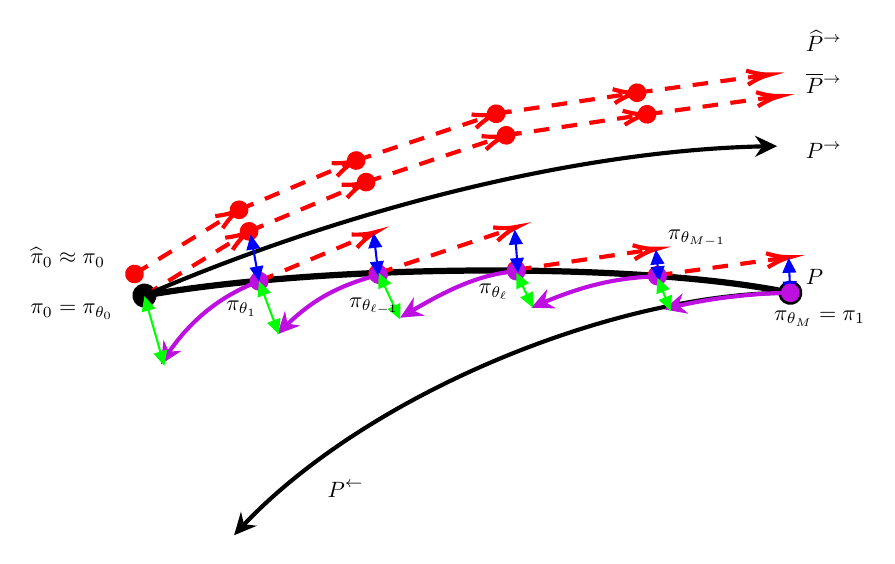
\begin{tikzpicture}[x=0.75pt,y=0.75pt,yscale=-0.8,xscale=0.8,every node/.style={scale=0.8}]
\draw [color={rgb, 255:red, 0; green, 0; blue, 0 }  ,draw opacity=1 ][line width=2.25]    (82,179.33) .. controls (190,160.33) and (379,158.67) .. (471,177.67) ;
\draw [shift={(471,177.67)}, rotate = 11.67] [color={rgb, 255:red, 0; green, 0; blue, 0 }  ,draw opacity=1 ][fill={rgb, 255:red, 0; green, 0; blue, 0 }  ,fill opacity=1 ][line width=2.25]      (0, 0) circle [x radius= 5.36, y radius= 5.36]   ;
\draw [shift={(82,179.33)}, rotate = 350.02] [color={rgb, 255:red, 0; green, 0; blue, 0 }  ,draw opacity=1 ][fill={rgb, 255:red, 0; green, 0; blue, 0 }  ,fill opacity=1 ][line width=2.25]      (0, 0) circle [x radius= 5.36, y radius= 5.36]   ;
\draw [color={rgb, 255:red, 255; green, 0; blue, 0 }  ,draw opacity=1 ][line width=1.5]  [dash pattern={on 5.63pt off 4.5pt}]  (82,179.33) -- (142.44,142.24) ;
\draw [shift={(145,140.67)}, rotate = 148.46] [color={rgb, 255:red, 255; green, 0; blue, 0 }  ,draw opacity=1 ][line width=1.5]    (14.21,-4.28) .. controls (9.04,-1.82) and (4.3,-0.39) .. (0,0) .. controls (4.3,0.39) and (9.04,1.82) .. (14.21,4.28)   ;
\draw [color={rgb, 255:red, 255; green, 0; blue, 0 }  ,draw opacity=1 ][line width=1.5]  [dash pattern={on 5.63pt off 4.5pt}]  (145,140.67) -- (212.73,112.16) ;
\draw [shift={(215.5,111)}, rotate = 157.18] [color={rgb, 255:red, 255; green, 0; blue, 0 }  ,draw opacity=1 ][line width=1.5]    (14.21,-4.28) .. controls (9.04,-1.82) and (4.3,-0.39) .. (0,0) .. controls (4.3,0.39) and (9.04,1.82) .. (14.21,4.28)   ;
\draw [shift={(145,140.67)}, rotate = 337.18] [color={rgb, 255:red, 255; green, 0; blue, 0 }  ,draw opacity=1 ][fill={rgb, 255:red, 255; green, 0; blue, 0 }  ,fill opacity=1 ][line width=1.5]      (0, 0) circle [x radius= 4.36, y radius= 4.36]   ;
\draw [color={rgb, 255:red, 255; green, 0; blue, 0 }  ,draw opacity=1 ][line width=1.5]  [dash pattern={on 5.63pt off 4.5pt}]  (215.5,111) -- (296.99,83.78) ;
\draw [shift={(299.83,82.83)}, rotate = 161.53] [color={rgb, 255:red, 255; green, 0; blue, 0 }  ,draw opacity=1 ][line width=1.5]    (14.21,-4.28) .. controls (9.04,-1.82) and (4.3,-0.39) .. (0,0) .. controls (4.3,0.39) and (9.04,1.82) .. (14.21,4.28)   ;
\draw [shift={(215.5,111)}, rotate = 341.53] [color={rgb, 255:red, 255; green, 0; blue, 0 }  ,draw opacity=1 ][fill={rgb, 255:red, 255; green, 0; blue, 0 }  ,fill opacity=1 ][line width=1.5]      (0, 0) circle [x radius= 4.36, y radius= 4.36]   ;
\draw [color={rgb, 255:red, 255; green, 0; blue, 0 }  ,draw opacity=1 ][line width=1.5]  [dash pattern={on 5.63pt off 4.5pt}]  (299.83,82.83) -- (381.7,70.61) ;
\draw [shift={(384.67,70.17)}, rotate = 171.51] [color={rgb, 255:red, 255; green, 0; blue, 0 }  ,draw opacity=1 ][line width=1.5]    (14.21,-4.28) .. controls (9.04,-1.82) and (4.3,-0.39) .. (0,0) .. controls (4.3,0.39) and (9.04,1.82) .. (14.21,4.28)   ;
\draw [shift={(299.83,82.83)}, rotate = 351.51] [color={rgb, 255:red, 255; green, 0; blue, 0 }  ,draw opacity=1 ][fill={rgb, 255:red, 255; green, 0; blue, 0 }  ,fill opacity=1 ][line width=1.5]      (0, 0) circle [x radius= 4.36, y radius= 4.36]   ;
\draw [color={rgb, 255:red, 255; green, 0; blue, 0 }  ,draw opacity=1 ][line width=1.5]  [dash pattern={on 5.63pt off 4.5pt}]  (384.67,70.17) -- (462.03,59.57) ;
\draw [shift={(465,59.17)}, rotate = 172.2] [color={rgb, 255:red, 255; green, 0; blue, 0 }  ,draw opacity=1 ][line width=1.5]    (14.21,-4.28) .. controls (9.04,-1.82) and (4.3,-0.39) .. (0,0) .. controls (4.3,0.39) and (9.04,1.82) .. (14.21,4.28)   ;
\draw [shift={(384.67,70.17)}, rotate = 352.2] [color={rgb, 255:red, 255; green, 0; blue, 0 }  ,draw opacity=1 ][fill={rgb, 255:red, 255; green, 0; blue, 0 }  ,fill opacity=1 ][line width=1.5]      (0, 0) circle [x radius= 4.36, y radius= 4.36]   ;
\draw [color={rgb, 255:red, 0; green, 0; blue, 0 }  ,draw opacity=1 ][line width=1.5]    (82,179.33) .. controls (186.94,133.79) and (334.02,91.19) .. (459.21,89.38) ;
\draw [shift={(463,89.33)}, rotate = 179.55] [fill={rgb, 255:red, 0; green, 0; blue, 0 }  ,fill opacity=1 ][line width=0.08]  [draw opacity=0] (13.4,-6.43) -- (0,0) -- (13.4,6.44) -- (8.9,0) -- cycle    ;
\draw [shift={(82,179.33)}, rotate = 336.54] [color={rgb, 255:red, 0; green, 0; blue, 0 }  ,draw opacity=1 ][fill={rgb, 255:red, 0; green, 0; blue, 0 }  ,fill opacity=1 ][line width=1.5]      (0, 0) circle [x radius= 4.36, y radius= 4.36]   ;
\draw [color={rgb, 255:red, 0; green, 0; blue, 0 }  ,draw opacity=1 ][line width=1.5]    (139.43,319.9) .. controls (215.61,237.81) and (366.59,177.34) .. (471,177.67) ;
\draw [shift={(471,177.67)}, rotate = 0.18] [color={rgb, 255:red, 0; green, 0; blue, 0 }  ,draw opacity=1 ][fill={rgb, 255:red, 0; green, 0; blue, 0 }  ,fill opacity=1 ][line width=1.5]      (0, 0) circle [x radius= 4.36, y radius= 4.36]   ;
\draw [shift={(136,323.67)}, rotate = 311.76] [fill={rgb, 255:red, 0; green, 0; blue, 0 }  ,fill opacity=1 ][line width=0.08]  [draw opacity=0] (13.4,-6.43) -- (0,0) -- (13.4,6.44) -- (8.9,0) -- cycle    ;
\draw [color={rgb, 255:red, 255; green, 0; blue, 0 }  ,draw opacity=1 ][line width=1.5]  [dash pattern={on 5.63pt off 4.5pt}]  (76,166.33) -- (136.44,129.24) ;
\draw [shift={(139,127.67)}, rotate = 148.46] [color={rgb, 255:red, 255; green, 0; blue, 0 }  ,draw opacity=1 ][line width=1.5]    (14.21,-4.28) .. controls (9.04,-1.82) and (4.3,-0.39) .. (0,0) .. controls (4.3,0.39) and (9.04,1.82) .. (14.21,4.28)   ;
\draw [shift={(76,166.33)}, rotate = 328.46] [color={rgb, 255:red, 255; green, 0; blue, 0 }  ,draw opacity=1 ][fill={rgb, 255:red, 255; green, 0; blue, 0 }  ,fill opacity=1 ][line width=1.5]      (0, 0) circle [x radius= 4.36, y radius= 4.36]   ;
\draw [color={rgb, 255:red, 255; green, 0; blue, 0 }  ,draw opacity=1 ][line width=1.5]  [dash pattern={on 5.63pt off 4.5pt}]  (139,127.67) -- (206.73,99.16) ;
\draw [shift={(209.5,98)}, rotate = 157.18] [color={rgb, 255:red, 255; green, 0; blue, 0 }  ,draw opacity=1 ][line width=1.5]    (14.21,-4.28) .. controls (9.04,-1.82) and (4.3,-0.39) .. (0,0) .. controls (4.3,0.39) and (9.04,1.82) .. (14.21,4.28)   ;
\draw [shift={(139,127.67)}, rotate = 337.18] [color={rgb, 255:red, 255; green, 0; blue, 0 }  ,draw opacity=1 ][fill={rgb, 255:red, 255; green, 0; blue, 0 }  ,fill opacity=1 ][line width=1.5]      (0, 0) circle [x radius= 4.36, y radius= 4.36]   ;
\draw [color={rgb, 255:red, 255; green, 0; blue, 0 }  ,draw opacity=1 ][line width=1.5]  [dash pattern={on 5.63pt off 4.5pt}]  (209.5,98) -- (290.99,70.78) ;
\draw [shift={(293.83,69.83)}, rotate = 161.53] [color={rgb, 255:red, 255; green, 0; blue, 0 }  ,draw opacity=1 ][line width=1.5]    (14.21,-4.28) .. controls (9.04,-1.82) and (4.3,-0.39) .. (0,0) .. controls (4.3,0.39) and (9.04,1.82) .. (14.21,4.28)   ;
\draw [shift={(209.5,98)}, rotate = 341.53] [color={rgb, 255:red, 255; green, 0; blue, 0 }  ,draw opacity=1 ][fill={rgb, 255:red, 255; green, 0; blue, 0 }  ,fill opacity=1 ][line width=1.5]      (0, 0) circle [x radius= 4.36, y radius= 4.36]   ;
\draw [color={rgb, 255:red, 255; green, 0; blue, 0 }  ,draw opacity=1 ][line width=1.5]  [dash pattern={on 5.63pt off 4.5pt}]  (293.83,69.83) -- (375.7,57.61) ;
\draw [shift={(378.67,57.17)}, rotate = 171.51] [color={rgb, 255:red, 255; green, 0; blue, 0 }  ,draw opacity=1 ][line width=1.5]    (14.21,-4.28) .. controls (9.04,-1.82) and (4.3,-0.39) .. (0,0) .. controls (4.3,0.39) and (9.04,1.82) .. (14.21,4.28)   ;
\draw [shift={(293.83,69.83)}, rotate = 351.51] [color={rgb, 255:red, 255; green, 0; blue, 0 }  ,draw opacity=1 ][fill={rgb, 255:red, 255; green, 0; blue, 0 }  ,fill opacity=1 ][line width=1.5]      (0, 0) circle [x radius= 4.36, y radius= 4.36]   ;
\draw [color={rgb, 255:red, 255; green, 0; blue, 0 }  ,draw opacity=1 ][line width=1.5]  [dash pattern={on 5.63pt off 4.5pt}]  (378.67,57.17) -- (456.03,46.57) ;
\draw [shift={(459,46.17)}, rotate = 172.2] [color={rgb, 255:red, 255; green, 0; blue, 0 }  ,draw opacity=1 ][line width=1.5]    (14.21,-4.28) .. controls (9.04,-1.82) and (4.3,-0.39) .. (0,0) .. controls (4.3,0.39) and (9.04,1.82) .. (14.21,4.28)   ;
\draw [shift={(378.67,57.17)}, rotate = 352.2] [color={rgb, 255:red, 255; green, 0; blue, 0 }  ,draw opacity=1 ][fill={rgb, 255:red, 255; green, 0; blue, 0 }  ,fill opacity=1 ][line width=1.5]      (0, 0) circle [x radius= 4.36, y radius= 4.36]   ;
\draw [color={rgb, 255:red, 255; green, 0; blue, 0 }  ,draw opacity=1 ][line width=1.5]  [dash pattern={on 5.63pt off 4.5pt}]  (151,170.67) -- (218.73,142.16) ;
\draw [shift={(221.5,141)}, rotate = 157.18] [color={rgb, 255:red, 255; green, 0; blue, 0 }  ,draw opacity=1 ][line width=1.5]    (14.21,-4.28) .. controls (9.04,-1.82) and (4.3,-0.39) .. (0,0) .. controls (4.3,0.39) and (9.04,1.82) .. (14.21,4.28)   ;
\draw [shift={(151,170.67)}, rotate = 337.18] [color={rgb, 255:red, 255; green, 0; blue, 0 }  ,draw opacity=1 ][fill={rgb, 255:red, 255; green, 0; blue, 0 }  ,fill opacity=1 ][line width=1.5]      (0, 0) circle [x radius= 4.36, y radius= 4.36]   ;
\draw [color={rgb, 255:red, 255; green, 0; blue, 0 }  ,draw opacity=1 ][line width=1.5]  [dash pattern={on 5.63pt off 4.5pt}]  (222.5,166) -- (303.99,138.78) ;
\draw [shift={(306.83,137.83)}, rotate = 161.53] [color={rgb, 255:red, 255; green, 0; blue, 0 }  ,draw opacity=1 ][line width=1.5]    (14.21,-4.28) .. controls (9.04,-1.82) and (4.3,-0.39) .. (0,0) .. controls (4.3,0.39) and (9.04,1.82) .. (14.21,4.28)   ;
\draw [shift={(222.5,166)}, rotate = 341.53] [color={rgb, 255:red, 255; green, 0; blue, 0 }  ,draw opacity=1 ][fill={rgb, 255:red, 255; green, 0; blue, 0 }  ,fill opacity=1 ][line width=1.5]      (0, 0) circle [x radius= 4.36, y radius= 4.36]   ;
\draw [color={rgb, 255:red, 255; green, 0; blue, 0 }  ,draw opacity=1 ][line width=1.5]  [dash pattern={on 5.63pt off 4.5pt}]  (305.83,163.83) -- (387.7,151.61) ;
\draw [shift={(390.67,151.17)}, rotate = 171.51] [color={rgb, 255:red, 255; green, 0; blue, 0 }  ,draw opacity=1 ][line width=1.5]    (14.21,-4.28) .. controls (9.04,-1.82) and (4.3,-0.39) .. (0,0) .. controls (4.3,0.39) and (9.04,1.82) .. (14.21,4.28)   ;
\draw [shift={(305.83,163.83)}, rotate = 351.51] [color={rgb, 255:red, 255; green, 0; blue, 0 }  ,draw opacity=1 ][fill={rgb, 255:red, 255; green, 0; blue, 0 }  ,fill opacity=1 ][line width=1.5]      (0, 0) circle [x radius= 4.36, y radius= 4.36]   ;
\draw [color={rgb, 255:red, 255; green, 0; blue, 0 }  ,draw opacity=1 ][line width=1.5]  [dash pattern={on 5.63pt off 4.5pt}]  (390.67,167.17) -- (468.03,156.57) ;
\draw [shift={(471,156.17)}, rotate = 172.2] [color={rgb, 255:red, 255; green, 0; blue, 0 }  ,draw opacity=1 ][line width=1.5]    (14.21,-4.28) .. controls (9.04,-1.82) and (4.3,-0.39) .. (0,0) .. controls (4.3,0.39) and (9.04,1.82) .. (14.21,4.28)   ;
\draw [shift={(390.67,167.17)}, rotate = 352.2] [color={rgb, 255:red, 255; green, 0; blue, 0 }  ,draw opacity=1 ][fill={rgb, 255:red, 255; green, 0; blue, 0 }  ,fill opacity=1 ][line width=1.5]      (0, 0) circle [x radius= 4.36, y radius= 4.36]   ;
\draw [color={rgb, 255:red, 189; green, 16; blue, 224 }  ,draw opacity=1 ][line width=1.5]    (318.87,184.96) .. controls (345.9,173.22) and (366.17,168.62) .. (391,167.67) ;
\draw [shift={(391,167.67)}, rotate = 357.8] [color={rgb, 255:red, 189; green, 16; blue, 224 }  ,draw opacity=1 ][fill={rgb, 255:red, 189; green, 16; blue, 224 }  ,fill opacity=1 ][line width=1.5]      (0, 0) circle [x radius= 4.36, y radius= 4.36]   ;
\draw [shift={(315,186.67)}, rotate = 335.85] [fill={rgb, 255:red, 189; green, 16; blue, 224 }  ,fill opacity=1 ][line width=0.08]  [draw opacity=0] (13.4,-6.43) -- (0,0) -- (13.4,6.44) -- (8.9,0) -- cycle    ;
\draw [color={rgb, 255:red, 189; green, 16; blue, 224 }  ,draw opacity=1 ][line width=1.5]    (239.63,190.52) .. controls (260.43,178.27) and (281.43,166.56) .. (306,164.67) ;
\draw [shift={(306,164.67)}, rotate = 355.6] [color={rgb, 255:red, 189; green, 16; blue, 224 }  ,draw opacity=1 ][fill={rgb, 255:red, 189; green, 16; blue, 224 }  ,fill opacity=1 ][line width=1.5]      (0, 0) circle [x radius= 4.36, y radius= 4.36]   ;
\draw [shift={(236,192.67)}, rotate = 329.42] [fill={rgb, 255:red, 189; green, 16; blue, 224 }  ,fill opacity=1 ][line width=0.08]  [draw opacity=0] (13.4,-6.43) -- (0,0) -- (13.4,6.44) -- (8.9,0) -- cycle    ;
\draw [color={rgb, 255:red, 189; green, 16; blue, 224 }  ,draw opacity=1 ][line width=1.5]    (164.81,199.79) .. controls (184.46,180.04) and (200.08,173.35) .. (223,166.67) ;
\draw [shift={(223,166.67)}, rotate = 343.74] [color={rgb, 255:red, 189; green, 16; blue, 224 }  ,draw opacity=1 ][fill={rgb, 255:red, 189; green, 16; blue, 224 }  ,fill opacity=1 ][line width=1.5]      (0, 0) circle [x radius= 4.36, y radius= 4.36]   ;
\draw [shift={(162,202.67)}, rotate = 313.67] [fill={rgb, 255:red, 189; green, 16; blue, 224 }  ,fill opacity=1 ][line width=0.08]  [draw opacity=0] (13.4,-6.43) -- (0,0) -- (13.4,6.44) -- (8.9,0) -- cycle    ;
\draw [color={rgb, 255:red, 189; green, 16; blue, 224 }  ,draw opacity=1 ][line width=1.5]    (94.32,216.97) .. controls (110.89,191.42) and (130.95,178.31) .. (151,170.67) ;
\draw [shift={(151,170.67)}, rotate = 339.15] [color={rgb, 255:red, 189; green, 16; blue, 224 }  ,draw opacity=1 ][fill={rgb, 255:red, 189; green, 16; blue, 224 }  ,fill opacity=1 ][line width=1.5]      (0, 0) circle [x radius= 4.36, y radius= 4.36]   ;
\draw [shift={(92,220.67)}, rotate = 301.26] [fill={rgb, 255:red, 189; green, 16; blue, 224 }  ,fill opacity=1 ][line width=0.08]  [draw opacity=0] (13.4,-6.43) -- (0,0) -- (13.4,6.44) -- (8.9,0) -- cycle    ;
\draw [color={rgb, 255:red, 0; green, 0; blue, 255 }  ,draw opacity=1 ][line width=0.75]    (146.53,145.62) -- (150.47,167.71) ;
\draw [shift={(151,170.67)}, rotate = 259.88] [fill={rgb, 255:red, 0; green, 0; blue, 255 }  ,fill opacity=1 ][line width=0.08]  [draw opacity=0] (8.93,-4.29) -- (0,0) -- (8.93,4.29) -- cycle    ;
\draw [shift={(146,142.67)}, rotate = 79.88] [fill={rgb, 255:red, 0; green, 0; blue, 255 }  ,fill opacity=1 ][line width=0.08]  [draw opacity=0] (8.93,-4.29) -- (0,0) -- (8.93,4.29) -- cycle    ;
\draw [color={rgb, 255:red, 0; green, 0; blue, 255 }  ,draw opacity=1 ][line width=0.75]    (220.34,144.65) -- (222.66,164.69) ;
\draw [shift={(223,167.67)}, rotate = 263.42] [fill={rgb, 255:red, 0; green, 0; blue, 255 }  ,fill opacity=1 ][line width=0.08]  [draw opacity=0] (8.93,-4.29) -- (0,0) -- (8.93,4.29) -- cycle    ;
\draw [shift={(220,141.67)}, rotate = 83.42] [fill={rgb, 255:red, 0; green, 0; blue, 255 }  ,fill opacity=1 ][line width=0.08]  [draw opacity=0] (8.93,-4.29) -- (0,0) -- (8.93,4.29) -- cycle    ;
\draw [color={rgb, 255:red, 0; green, 0; blue, 255 }  ,draw opacity=1 ][line width=0.75]    (305.23,142.66) -- (306.77,162.68) ;
\draw [shift={(307,165.67)}, rotate = 265.6] [fill={rgb, 255:red, 0; green, 0; blue, 255 }  ,fill opacity=1 ][line width=0.08]  [draw opacity=0] (8.93,-4.29) -- (0,0) -- (8.93,4.29) -- cycle    ;
\draw [shift={(305,139.67)}, rotate = 85.6] [fill={rgb, 255:red, 0; green, 0; blue, 255 }  ,fill opacity=1 ][line width=0.08]  [draw opacity=0] (8.93,-4.29) -- (0,0) -- (8.93,4.29) -- cycle    ;
\draw [color={rgb, 255:red, 0; green, 0; blue, 255 }  ,draw opacity=1 ][line width=0.75]    (390.31,154.65) -- (391.69,167.68) ;
\draw [shift={(392,170.67)}, rotate = 263.99] [fill={rgb, 255:red, 0; green, 0; blue, 255 }  ,fill opacity=1 ][line width=0.08]  [draw opacity=0] (8.93,-4.29) -- (0,0) -- (8.93,4.29) -- cycle    ;
\draw [shift={(390,151.67)}, rotate = 83.99] [fill={rgb, 255:red, 0; green, 0; blue, 255 }  ,fill opacity=1 ][line width=0.08]  [draw opacity=0] (8.93,-4.29) -- (0,0) -- (8.93,4.29) -- cycle    ;
\draw [color={rgb, 255:red, 0; green, 0; blue, 255 }  ,draw opacity=1 ][line width=0.75]    (470.13,159.66) -- (470.87,176.67) ;
\draw [shift={(471,179.67)}, rotate = 267.51] [fill={rgb, 255:red, 0; green, 0; blue, 255 }  ,fill opacity=1 ][line width=0.08]  [draw opacity=0] (8.93,-4.29) -- (0,0) -- (8.93,4.29) -- cycle    ;
\draw [shift={(470,156.67)}, rotate = 87.51] [fill={rgb, 255:red, 0; green, 0; blue, 255 }  ,fill opacity=1 ][line width=0.08]  [draw opacity=0] (8.93,-4.29) -- (0,0) -- (8.93,4.29) -- cycle    ;
\draw [color={rgb, 255:red, 0; green, 255; blue, 0 }  ,draw opacity=1 ][line width=0.75]    (82.82,182.55) -- (93.18,218.78) ;
\draw [shift={(94,221.67)}, rotate = 254.05] [fill={rgb, 255:red, 0; green, 255; blue, 0 }  ,fill opacity=1 ][line width=0.08]  [draw opacity=0] (8.93,-4.29) -- (0,0) -- (8.93,4.29) -- cycle    ;
\draw [shift={(82,179.67)}, rotate = 74.05] [fill={rgb, 255:red, 0; green, 255; blue, 0 }  ,fill opacity=1 ][line width=0.08]  [draw opacity=0] (8.93,-4.29) -- (0,0) -- (8.93,4.29) -- cycle    ;
\draw [color={rgb, 255:red, 0; green, 255; blue, 0 }  ,draw opacity=1 ][line width=0.75]    (152.05,173.48) -- (161.95,199.86) ;
\draw [shift={(163,202.67)}, rotate = 249.44] [fill={rgb, 255:red, 0; green, 255; blue, 0 }  ,fill opacity=1 ][line width=0.08]  [draw opacity=0] (8.93,-4.29) -- (0,0) -- (8.93,4.29) -- cycle    ;
\draw [shift={(151,170.67)}, rotate = 69.44] [fill={rgb, 255:red, 0; green, 255; blue, 0 }  ,fill opacity=1 ][line width=0.08]  [draw opacity=0] (8.93,-4.29) -- (0,0) -- (8.93,4.29) -- cycle    ;
\draw [color={rgb, 255:red, 0; green, 255; blue, 0 }  ,draw opacity=1 ][line width=0.75]    (224.26,168.39) -- (234.74,190.95) ;
\draw [shift={(236,193.67)}, rotate = 245.1] [fill={rgb, 255:red, 0; green, 255; blue, 0 }  ,fill opacity=1 ][line width=0.08]  [draw opacity=0] (8.93,-4.29) -- (0,0) -- (8.93,4.29) -- cycle    ;
\draw [shift={(223,165.67)}, rotate = 65.1] [fill={rgb, 255:red, 0; green, 255; blue, 0 }  ,fill opacity=1 ][line width=0.08]  [draw opacity=0] (8.93,-4.29) -- (0,0) -- (8.93,4.29) -- cycle    ;
\draw [color={rgb, 255:red, 0; green, 255; blue, 0 }  ,draw opacity=1 ][line width=0.75]    (307.29,168.38) -- (314.71,183.96) ;
\draw [shift={(316,186.67)}, rotate = 244.54] [fill={rgb, 255:red, 0; green, 255; blue, 0 }  ,fill opacity=1 ][line width=0.08]  [draw opacity=0] (8.93,-4.29) -- (0,0) -- (8.93,4.29) -- cycle    ;
\draw [shift={(306,165.67)}, rotate = 64.54] [fill={rgb, 255:red, 0; green, 255; blue, 0 }  ,fill opacity=1 ][line width=0.08]  [draw opacity=0] (8.93,-4.29) -- (0,0) -- (8.93,4.29) -- cycle    ;
\draw [color={rgb, 255:red, 189; green, 16; blue, 224 }  ,draw opacity=1 ][line width=1.5]    (399.19,186.55) .. controls (423.58,180.35) and (453.99,177.67) .. (471,177.67) ;
\draw [shift={(471,177.67)}, rotate = 0] [color={rgb, 255:red, 189; green, 16; blue, 224 }  ,draw opacity=1 ][fill={rgb, 255:red, 189; green, 16; blue, 224 }  ,fill opacity=1 ][line width=1.5]      (0, 0) circle [x radius= 4.36, y radius= 4.36]   ;
\draw [shift={(395,187.67)}, rotate = 344.36] [fill={rgb, 255:red, 189; green, 16; blue, 224 }  ,fill opacity=1 ][line width=0.08]  [draw opacity=0] (13.4,-6.43) -- (0,0) -- (13.4,6.44) -- (8.9,0) -- cycle    ;
\draw [color={rgb, 255:red, 0; green, 255; blue, 0 }  ,draw opacity=1 ][line width=0.75]    (392.11,171.45) -- (397.89,185.88) ;
\draw [shift={(399,188.67)}, rotate = 248.2] [fill={rgb, 255:red, 0; green, 255; blue, 0 }  ,fill opacity=1 ][line width=0.08]  [draw opacity=0] (8.93,-4.29) -- (0,0) -- (8.93,4.29) -- cycle    ;
\draw [shift={(391,168.67)}, rotate = 68.2] [fill={rgb, 255:red, 0; green, 255; blue, 0 }  ,fill opacity=1 ][line width=0.08]  [draw opacity=0] (8.93,-4.29) -- (0,0) -- (8.93,4.29) -- cycle    ;

\draw (12,183.33) node [anchor=north west][inner sep=0.75pt]   [align=left] {$\displaystyle \pi _{0} =\pi _{\theta _{0}}$};
\draw (130,181.33) node [anchor=north west][inner sep=0.75pt]   [align=left] {$\displaystyle \pi _{\theta _{1}}$};
\draw (396,138.33) node [anchor=north west][inner sep=0.75pt]   [align=left] {$\displaystyle \pi _{\theta _{M-1}}$};
\draw (460,187.33) node [anchor=north west][inner sep=0.75pt]   [align=left] {$\displaystyle \pi _{\theta _{M}} =\pi _{1}$};
\draw (191,290.33) node [anchor=north west][inner sep=0.75pt]   [align=left] {$\displaystyle \mathbb{P}^{\leftarrow }$};
\draw (479,86.33) node [anchor=north west][inner sep=0.75pt]   [align=left] {$\displaystyle \mathbb{P^{\rightarrow }}$};
\draw (479,44.33) node [anchor=north west][inner sep=0.75pt]   [align=left] {$\displaystyle \overline{\mathbb{P}}\mathbb{^{\rightarrow }}$};
\draw (479,162.33) node [anchor=north west][inner sep=0.75pt]   [align=left] {$\displaystyle \mathbb{P}$};
\draw (479,18.33) node [anchor=north west][inner sep=0.75pt]   [align=left] {$\displaystyle \mathbb{\widehat{P}^{\rightarrow }}$};
\draw (12,149.33) node [anchor=north west][inner sep=0.75pt]   [align=left] {$\displaystyle \widehat{\pi }_{0} \approx \pi _{0}$};
\draw (204,179.33) node [anchor=north west][inner sep=0.75pt]   [align=left] {$\displaystyle \pi _{\theta _{\ell -1}}$};
\draw (282,171.33) node [anchor=north west][inner sep=0.75pt]   [align=left] {$\displaystyle \pi _{\theta _{\ell }}$};

\end{tikzpicture}
    \caption{
    Illustration of the proof idea for \cref{thm:ais_complexity}.}
    \label{fig:prf_idea}
\end{figure}

\begin{enumerate}[wide=0pt,itemsep=0pt, topsep=0pt,parsep=0pt,partopsep=0pt]
    \item Analogously to the analysis of JE (\cref{thm:jar_complexity}), define the reference path measure $\P$ with transition kernels $F^*_\l$ such that $x_\l\sim\pi_{\theta_\l}$.
    Given the sampling path measure $\Phr$, define $\Pbr$ as the version of $\Phr$ without the initialization error, i.e., by replacing $\pih_0$ with $\pi_0$ in \cref{eq:ais_phr}. 
    \item Show that it suffices to obtain an accurate estimate $\Zh_0$ and initialization distribution $\pih_0$, together with sufficiently small KL divergences $\kl(\P\|\Pl)$ and $\kl(\P\|\Pbr)$, which quantify the closeness between the continuous dynamics and the discretization error in implementation, respectively.
    \item Using the chain rule, decompose $\kl(\P\|\Pl)$ into the sum of KL divergences between each pair of transition kernels $F_\l$ and $F^*_\l$ (i.e., the sum of \green{green} ``distances''). As in the proof of the convergence of JE (\cref{thm:jar_complexity}), $F^*_\l$, a transition kernel from $\pi_{\theta_{\l-1}}$ to $\pi_{\theta_\l}$, is realized by ALD with a compensatory vector field, ensuring the SDE exactly follows the trajectory $(\pi_\theta)_{\theta\in[\theta_{\l-1},\theta_\l]}$. 
    Similarly, by applying the chain rule and Girsanov theorem, we can express $\kl(\P\|\Pbr)$ as the sum of the \blue{blue} ``distances'', allowing for a similar analysis.
    \item Finally, derive three necessary conditions on the time steps $\theta_{\l}$ to control both $\kl(\P\|\Pl)$ and $\kl(\P\|\Pbr)$. Choosing a proper schedule yields the desired complexity bound.
\end{enumerate}

Our proposed algorithm consists of two phases: first, estimating $Z_0$ by TI, which is provably efficient for well-conditioned distributions, and second, estimating $Z$ by AIS, which is better suited for handling non-log-concave distributions. 
The three terms in \cref{eq:ais_complexity} arise from (i) ensuring the accuracy of $\Zh_0$, (ii) controlling $\kl(\P\|\Pl)$, and (iii) controlling $\kl(\P\|\Pbr)$, respectively, as discussed in \textbf{2.} above.
Due to the non-log-concavity of $\pi$, the action $\cA$ is typically large, making (iii), the cost for controlling the discretization error, the dominant complexity.
Finally, the $\varepsilon$-dependence can be interpreted as the total duration $T=\Theta\ro{\frac{1}{\varepsilon^2}}$ required for the continuous dynamics to converge (as in \cref{thm:jar_complexity}) divided by the step size $\Thetat(\varepsilon^2)$ to control the discretization error.